\documentclass[a4paper,11pt,uplatex]{jsarticle}
\usepackage{amsmath,amssymb}
\usepackage{bm}
\usepackage[dvipdfmx]{graphicx}
\usepackage{here}
\usepackage{longtable}

%テキストの表示領域の調節
\setlength{\textwidth}{\paperwidth}
\addtolength{\textwidth}{-40truemm}
\setlength{\textheight}{\paperheight}
\addtolength{\textheight}{-45truemm}

%余白の調節
\setlength{\topmargin}{-10.4truemm}
\setlength{\evensidemargin}{-5.4truemm}
\setlength{\oddsidemargin}{-5.4truemm}
\setlength{\headheight}{17pt}
\setlength{\headsep}{10mm}
\addtolength{\headsep}{-17pt}
\setlength{\footskip}{5mm}

% \nofiles
\begin{document}
\section{目的}
工業製品は適切な温度状態に保たれなければならない.例えば,コンピュータのCPUは稼働中に多量の熱を発するため,うまく放熱されない場合には温度が上昇し続けて物理的に演算のできない状態に陥る.したがって,効率よく放熱処理を施すことは必須である.ここでは,熱移動の基本形式の一つである対流熱伝達について理解を深める.
\section{原理}
空気や水などの流体内に温度差が生じると熱膨張による密度差によって流体に運動が発生する.このような現象を自然対流と呼ぶ.
静止した空気中に高温物体を設置すると壁近傍に熱せられた空気の層(温度境界層)が生じ,浮力によってそうないの空気が上方に流動して熱を運んでいく.このような電熱形式を自然対流熱伝達という.
\par
一方,外部からの仕事によって発生する流体の運動は強制対流と呼ぶ.またこの時に行われる熱移動を強制熱対流伝達と呼ぶ.


\par
物体の壁面温度を$T_w$[K],流体の壁より十分離れた位置における温度を$T_0$[K],面積$A[\mathrm{m^2}]$の物体表面より単位時間当たりに放出される熱量を$Q$[W]とすると,$Q$は一般的に以下のように表される.
\begin{align}
  Q=hA(T_w-T_0)
\end{align}
上式で定義される$h$[W/($\mathrm{m^2}$K)]を熱伝達率と呼ぶ.$h$の値は対流の種類や強さ,流体の種類によって変化するが,通常の条件下では以下の範囲になる.
\begin{table}[H]
\begin{tabular}{lrrl}
静止気体中の自然対流 & 1-    & 25     &  W/($\mathrm{m^2}K$)\\
気体の強制対流    & 10-   & 250    &  W/($\mathrm{m^2}K$)\\
液体の強制対流    & 150-  & 5000   &  W/($\mathrm{m^2}K$)\\
相変化(沸騰・凝縮) & 1000- & 250000 & W/($\mathrm{m^2}K$)
\end{tabular}
\end{table}
自然対流による熱伝達率はかなり小さい.このため自然対流熱伝達によって放熱を行う場合には,高温側側面にフィンを設けて放熱量の増大を計ることが多い.
\par
まず,フィンの設置によってどの程度$Q$が増加するかを単純な一枚フィンの場合について考察する.
\par
定常状態の条件下でフィンの根元を$x$軸の原点にとり,任意断面$x$における微小区間$dx$に対する熱収支を考慮すると式(2)が導かれる.
\begin{align}
  \label{式2}
  \left( \frac{d}{dx}\right) \left(kS \frac{dT}{dx}\right)dx - hRdx(T-T_0)=0
\end{align}
ただし,
\begin{table}[H]
\begin{tabular}{ll}
$k$:フィンの熱伝達率 & ($k = 428$ W/(mK):銅) \\
$R$:フィン断面の接触長 & ($2 \times (b+L)$) \\
$S$:フィン断面積 & ($b \times L$) \\
$T$:$x=x$におけるフィン温度 & \\
$T_0$:周囲の空気温度 & \\
$h$:フィン表面の熱伝達率 &
\end{tabular}
\end{table}
$k,S,T_0,h=\mathrm{const}$とすると,式(\ref{式2})は$T$に関する二階の常微分方程式(\ref{式3})となる.
\begin{align}
  \label{式3}
  \frac{d^2T}{dx^2} - \left(\frac{hR}{kS}\right)(T-T_0)=0
\end{align}
式(\ref{式3})の解は,$T=T_w$ at $x=0$及び,$dT/dx=0$ at $x=H$となる境界条件より,次式のように表される.
\begin{align}
  \label{式4}
  \frac{T-T_0}{T_w-T_0}=\frac{\cosh{B(H-x)}}{\cosh{BH}}
\end{align}
ただし,
\begin{align}
  B=\sqrt{\frac{hR}{kS}}
\end{align}
式(\ref{式4})で得られた温度分布$T=T(x)$により,一枚のフィンからの放熱量$Q$は次式で与えられる.
\begin{align}
  \label{式6}
  Q &= \int^H_0 hR(T-T_0)dx \\
  &= \sqrt{\frac{hR}{kS}}(T_w-T_0)\tanh{BH}
\end{align}
また,$Q$は次式で定義される基板からフィンに流入する熱量に等しい.
\begin{align}
  Q=-kS\left(\frac{dT}{dx}\right)_{x=0}
\end{align}

\par
次に,フィンをつけたことによる放熱量の増加分について検討する.フィンがない場合(接触面積 $=S$)の放熱量を$Q_0$とし,フィンをつけた場合(接触面積$=RH$の放熱量)$Q$との比を$\varepsilon$とすると,
\begin{align}
  \varepsilon = \frac{Q}{Q_0} = \sqrt{\frac{kR}{hS}}\tanh{BH}
\end{align}

となる.$\varepsilon$はフィン有効係数と呼ばれる.
\par
以上の結果より,$N$枚のフィンによる放熱量$Q_N$は式(\ref{式6})による$Q$を用いて次式で与えられる.
\begin{align}
  \label{式9}
  Q_N = N(hA_w(T_w-T_0)+Q) \simeq NQ
\end{align}
ただし,$A_w$はフィンの表面以外での流体との接触面積$PL$であり,フィンと空気との接触面積$A_f = 2HL$に比べて省略できるものとする.
ここで,式(\ref{式6})と式(\ref{式9})は,$Q_N$を大きくするためにはフィンの熱伝導率$k$,枚数$N$,高さ$H$を大きくし,厚さ$b$を小さくすれば良いことを示している.
\par
なお,フィン枚数$N$を大きくすると,フィン相互間の干渉が強くなり,式(\ref{式6})が適用できなくなる.また,ここではフィン表面の熱伝達率$h$を一定と仮定している,実際には$h=h(x)$であり,さらにフィンのピッチ,姿勢によってフィン周囲の流れは大きく変化する.
本実験では,自然対流場において,複数フィンに対する熱伝達率$h$がフィンの姿勢によりどのように変化するかを実験的に求め,また強制対流が加わった場合に熱伝達率について合わせて検討した.

\section{方法}
図\ref{実験装置断面図},\ref{フィン設置状態}に実験装置の概略を示す.銅製基盤の寸法は$40.0 \times 42.0$であり,厚さ$b=1.7$[mm],ピッチ$P=4.37$[mm],高さ$H=35.0$[mm],及び枚数$N=7$のフィンに対して実験を行った.
\par
まずフィン基板を水平に設置し(この状態での回転角$\theta$を零にとる),加熱量一定の条件下でフィンを加熱した.フィン基板の平衡温度が100-150$^\circ$Cとなるように,
ヒータの出力を調整してフィンの基板温度の時間的変化を調べた.基板温度の平均値$T_{wm}$と雰囲気の温度$T_0$との差が安定するまで測定を行った.
次に,フィン基板の回転角$\theta$を45$^\circ$変化させて$\theta=45^\circ,90^\circ,135^\circ,180^\circ$において同様の測定を繰り返した.
\par
次に$180^\circ$の状態において,送風機の電源をを入れ,一定流量の空気を流し自然対流時と同様に$T_{wm}$と$T_0$との差が安定するまで測定を行った.
\begin{figure}[H]
  \begin{center}
    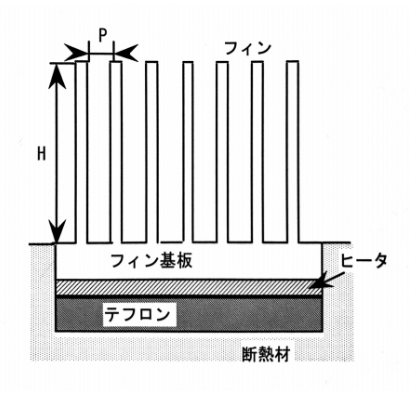
\includegraphics[width = 10cm]{画像/fig1.png}
    \caption{実験装置断面図}
    \label{実験装置断面図}
  \end{center}
\end{figure}
\begin{figure}[H]
  \begin{center}
    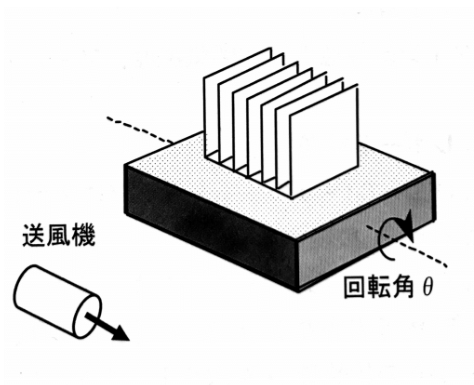
\includegraphics[width = 10cm]{画像/fig2.png}
    \caption{フィン設置状態}
    \label{フィン設置状態}
  \end{center}
\end{figure}
\par
実験は加熱量一定の条件下で行うので,フィン基板回転角$\theta$がある値での,定常状態における基板平均温度と雰囲気温度との差は次式を満足する.
\begin{align}
  IE = hA_f (T_{wm}- T_0)
\end{align}
よって,フィン表面の平均熱伝達率$h$[W/$(\mathrm{m}^2 \mathrm{K})$]を求めることができる.
\begin{align}
  h=\frac{IE}{A_f(T_{wm}-T_0)}
\end{align}
ここで,
\begin{description}
  \item[$I$] ヒータ電流[A]
  \item[$E$] ヒータ電圧[V]
  \item[$A_f$] フィン表面積$=2NHL$[m$^2$]
\end{description}
\section{結果}
測定結果はレポート末尾に添付した.また,測定結果を元に$T_{wm}−T_0$の時間変化を示したグラフ(図3)を作成し,レポート末尾に添付した.
次に,各$\theta$の値における平均熱伝達率$h$を求め、表を作成した.
なお、$T_{wm}−T_0$の平均は各角度において温度が安定している下から三点の平均とした.作成した表を以下の表1に示す.
\begin{table}[H]
\begin{center}
\caption{フィンの角度$\theta$における平均熱伝達率$h$}
\begin{tabular}{lll}
$\theta$[$^\circ$]& $T_{wm}-T_0$[$^\circ$C] & $h$[W/$(\mathrm{m}^2 \mathrm{K})$] \\ \hline
0 & 78.63 &  17.00 \\ \hline
45 & 79.33 & 16.85\\ \hline
90 & 67.23 & 19.89 \\ \hline
135 & 66.63 & 20.07 \\ \hline
180 & 68.43 & 19.54 \\ \hline
強制対流 & 40.3 & 33.18 \\ \hline
\end{tabular}
\end{center}
\end{table}
\section{考察及び課題}
課題1,2については結果において示した.
\subsection{課題3}
(2)式および(4)式を導出する.位置$x$でフィンの熱伝導により流入する熱量$\dot{Q_x}$は、フーリエの法則を用いて次のように表される.
\begin{align}
  \dot{Q_x}=-Sk \frac{dT}{dx}
\end{align}
また,位置$x+dx$においてフィンの熱伝導により流出する熱量$\dot{Q}_{x+dx}$は同様に考えると,
\begin{align}
  \dot{Q_x}=-S \left(k \frac{dT}{dx}\right)_{x+dx} = -S\left[ \left(k \frac{dT}{dx} \right) + \frac{d}{dx} \left(k \frac{dT}{dx}\right)dx \right]
\end{align}
ここで,フィンの表面から空気中へ対流熱伝達により放出される伝熱量$d \dot{Q_f}$を考慮する.フィン断面の接触長は$R$,またフィンの熱伝達率は$h$であるから,
表面$Rdx$から放出される伝熱量$d \dot{Q_f}$は
\begin{align}
  d \dot{Q_f}= h(T-T_0)Rdx
\end{align}
と表せる.
定常状態においてはフィンに流入する伝熱量と流出する伝熱量は等しくなるので,次の式が成り立つ.
\begin{align}
  \dot{Q_x}-\dot{Q}_{x+dx}-d \dot{Q_f}=0
\end{align}
よって、(16)式に(13)(14)(15)式を代入すると、(2)式が導出される.
\begin{align}
  -S\left(k \frac{dT}{dx} \right) +S\left[ \left(k \frac{dT}{dx} \right) + \frac{d}{dx} \left(k \frac{dT}{dx}\right)dx \right] -h(T-T_0)Rdx =0 \\
  \left( \frac{d}{dx}\right) \left[ kS \frac{dT}{dx} \right]dx -hRdx(T-T_0) =0
\end{align}
続いて,(2)式を変形した(3)式において$(hR/kS) =B^2,T−T0=\theta$とおくと、(3)式は次のように表される.
\begin{align}
  \frac{d^2\theta}{dx^2} - B^2\theta =0
\end{align}
ここで,$T_0$は定数なので省略した.この微分方程式の一般解は,
\begin{align}
  \theta = C_1 e^{Bx} + C_2 e^{-Bx}
\end{align}
と表せる.境界条件$T=T_{w}(x−0),dT/dx=0(x=H)$より,$C_1$,$C_2$の値は
\begin{align}
  C_1 &= \frac{T_w - T_0}{2\cosh BH} e^{-BH} \\
  C_2 &= \frac{T_w - T_0}{2\cosh BH} e^{BH}
\end{align}
と求まるので,$(T−T_0)/(T_W−T_0)$に$\theta$を代入することで、(4)式が導出される.
\begin{align}
  \frac{T-T_0}{T_w-T_0} &= \frac{\theta}{T_w-T_0} = \frac{C_1e^{Bx} + C_2e^{-Bx}}{T_w-T_0} \\
  &= \frac{\cosh B(H-x)}{\cosh BH}
\end{align}

\subsection{課題4}
$\theta$ = 90$^\circ$での平均熱伝達率$h$= 19.89[W/m$^2$K]を用いて、(6)式から$\theta$ = 90$^\circ$におけるフィン一枚あたりの放熱量$Q$を求めると,$Q$= 3.815[W]と求められた.
さらに,フィンの枚数$N$は$N$= 7であるため,フィン全体の放熱量$NQ$は$NQ$= 26.71[W]となる.
一方ヒーターの発熱量$IE$は$IE$= 0.78×33.6 =26.21[W]となり、フィンからの放熱量の方がヒーターの発熱量よりわずかに大きくなった.
つまり,フィンを複数枚にした時,一枚の時よりも放熱量が低下するということである.
フィンが複数枚になると,フィンの近くに放熱源が増えること,さらに周囲の空気の流れが少なくなることを間接的に意味しており,
放熱源が付近に存在する場合としない場合では,放熱量に差が出ると考えられる.
そこで,7枚のフィンの両端の部分を切り取り,そこでは一枚の場合と同じ放熱量であると考えると,互いに熱が干渉するフィンは6枚分となる.
すると,ヒーターの発熱量からフィン1枚あたりの発熱量を引き,6で除すると,干渉時のヒーターの発熱量が求められるはずである.
$(IE - Q)/6= 3.732$[W]となり,これが干渉時のフィンの一枚あたりの放熱量であると推測される.
\subsection{課題5}
$\theta$に依存して$h$がなぜ変化するのかを検討する.熱伝達率は自然対流に影響されるが,この自然対流は非常に僅かな対流なので,空気の流れが妨げられたりすることでも$h$の値は大きく変化することになる.
表1を見ると最も熱伝達率が大きくなったのは$\theta$= 135$^\circ$であったが,これは自然対流の流れの方向と関係していると思われる.
一般に,熱が発生すると,上昇気流が生じ,空気は下から上へと移動しようとする,
その際に上下方向の経路がある場合の方がより対流が起こりやすいと考えられる.
\subsection{課題6}
強制対流時の熱伝達率と,同じ姿勢である$\theta$= 180$^\circ$での熱伝達率を比較すると,強制対流時の熱伝達率の方が自然対流時のものより約1.70倍大きな値となっていることがわかる.
これは強制的に流れを作ることで自然対流に比べて多くの空気がフィンと接触することができ,フィンから奪える熱が多くなったからだと思われる.
フィンに対してより多くの空気を送り込み,滑らかに排出させ,対流させることが放熱に重要であることがわかる.
つまり,表面積をできるだけ大きくし,かつ対流を妨げずにスムーズに流すことができる形状であることが効率的な放熱促進装置として配慮すべき点であると考えられる.
\subsection{課題7}
\subsubsection{熱電対温度計}
\begin{description}
  \item[原理] 熱電対温度計ではゼーベック効果を用いることで温度を測る計測法である.
  ゼーベック効果とは,異なる材料の2本の金属線を接続して1つの回路,すなわち熱電対をつくり,2つの接点に温度差を与えることで
  回路に電圧が発生する現象のことである.
  この現象は、1821年にドイツの物理学者トーマス・ゼーベックによって発見されたことに由来している.
  片端を解放することによって,電位差,いわゆる熱起電力が堅守される.熱起電力は,組み合わせる金属の種類と両接点の温度差には依存するが,
  構成する2つの金属の形状と大きさには関係しない.この現象を利用したものが熱電対である.
  熱電対には以下の3つの法則がある.
  \begin{description}
    \item[均質回路の法則] 同じ金属線(均質な金属)のみでは,熱電対として熱起電力を取り出せないと言う法則.
    同種の金属構成された場合,熱電対にはなり得ない.
    \item[中間金属の法則] 熱電対の間に異種金属が挿入された際,その両端に温度差がない場合は,温度計測に影響を受けない.
    挿入された異種金属間に温度差が生じた場合,誤差の原因となる.
    \item[中間温度の法則] 回路中の中間温度が既知である場合,温接点,中間温度,基準接点それぞれの温度差から得た起電力の和と全体の起電力は等しい,という法則.
  \end{description}
  \item [特長] 熱電対温度計には以下のような特長がある.
  \begin{itemize}
    \item 熱起電力が大きく,特性のバラツキが小さく互換性がある.
    \item 高温または低温で使用しても,熱起電力が安定で寿命が長い.
    \item 耐熱性が高く,高温においても機械的強度が保たれている.
    \item 耐食性が高く,ガスなどに対しても丈夫.
  \end{itemize}
  \newpage
  \item [精度] 熱電対温度計はJISで構成材料および階級による精度の許容差が規定されている.以下にはJISで規定される熱電対の精度を示す.
  \begin{figure}[H]
    \begin{center}
      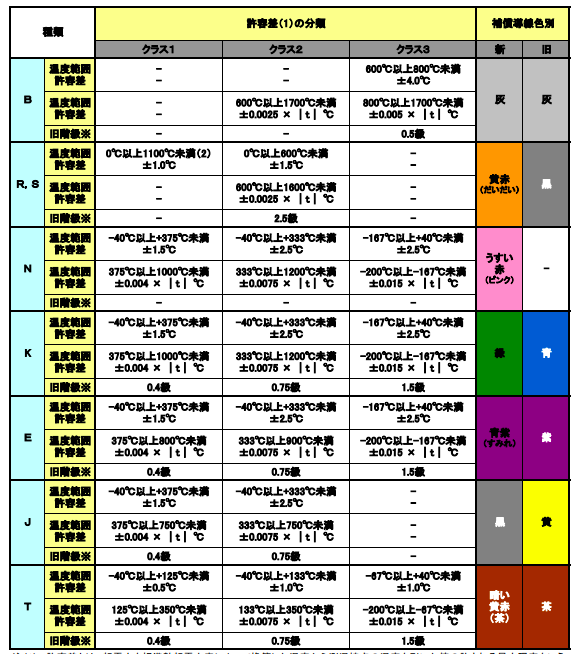
\includegraphics[width = 10cm]{画像/熱電対.png}
      \caption{熱電対のJIS規格}
      \label{熱電対のJIS規格}
    \end{center}
  \end{figure}
\end{description}






\section{付録}
\begin{longtable}{lllll}
\caption{実験から得られた測定値} \\
角度$[^\circ]$ & 時間 & $T_{wm}$ & $T_0$ & $T_w-T_0$ \\ \hline

\endfirsthead

0 & 0 & 98.7 & 20.6 & 78.1 \\ \hline
 & 1 & 98.9 & 20.6 & 78.3 \\ \hline
 & 2 & 98.9 & 20.6 & 78.3 \\ \hline
 & 3 & 99.1 & 20.7 & 78.4 \\ \hline
 & 4 & 99.1 & 20.7 & 78.4 \\ \hline
 & 5 & 99.2 & 20.7 & 78.5 \\ \hline
 & 6 & 99.3 & 20.7 & 78.6 \\ \hline
 & 7 & 99.3 & 20.7 & 78.6 \\ \hline
 & 8 & 99.4 & 20.7 & 78.7 \\ \hline
 & 9 & 99.4 & 20.8 & 78.6 \\ \hline
 & 10 & 99.4 & 20.7 & 78.7 \\ \hline
45 & 11 & 99 & 20.8 & 78.2 \\ \hline
 & 12 & 99.3 & 20.8 & 78.5 \\ \hline
 & 13 & 99.5 & 20.8 & 78.7 \\ \hline
 & 14 & 99.6 & 20.9 & 78.7 \\ \hline
 & 15 & 99.8 & 20.9 & 78.9 \\ \hline
 & 16 & 99.9 & 20.9 & 79 \\ \hline
 & 17 & 100 & 20.9 & 79.1 \\ \hline
 & 18 & 100.2 & 20.9 & 79.3 \\ \hline
 & 19 & 100.3 & 21.0 & 79.3 \\ \hline
 & 20 & 100.4 & 21.0 & 79.4 \\ \hline
90 & 21 & 99.5 & 20.9 & 78.6 \\ \hline
 & 22 & 98 & 21.0 & 77 \\ \hline
 & 23 & 96.6 & 21.0 & 75.6 \\ \hline
 & 24 &  &  &  \\ \hline
 & 25 & 94.4 & 21.0 & 73.4 \\ \hline
 & 26 & 93.5 & 21.0 & 72.5 \\ \hline
 & 27 & 92.7 & 21.0 & 71.7 \\ \hline
 & 28 & 92.1 & 21.0 & 71.1 \\ \hline
 & 29 & 91.4 & 21.0 & 70.4 \\ \hline
 & 30 & 91 & 21.1 & 69.9 \\ \hline
 & 31 & 90.5 & 21.1 & 69.4 \\ \hline
 & 32 & 90.1 & 21.1 & 69.0 \\ \hline
 & 33 & 89.7 & 21.1 & 68.6 \\ \hline
 & 34 & 89.3 & 21.1 & 68.2 \\ \hline
 & 35 & 89 & 21.1 & 67.9 \\ \hline
 & 36 & 88.8 & 21.1 & 67.7 \\ \hline
 & 37 & 88.6 & 21.1 & 67.5 \\ \hline
 & 38 & 88.3 & 21.1 & 67.2 \\ \hline
 & 39 & 88.2 & 21.2 & 67.0 \\ \hline
 & 40 & 88 & 21.2 & 66.8 \\ \hline
 & 41 & 87.9 & 21.1 & 66.8 \\ \hline
135 & 42 & 89.3 & 21.2 & 68.1 \\ \hline
 & 43 & 89.1 & 21.1 & 68.0 \\ \hline
 & 44 & 88.8 & 21.2 & 67.6 \\ \hline
 & 45 & 88.5 & 21.2 & 67.3 \\ \hline
 & 46 & 88.3 & 21.2 & 67.1 \\ \hline
 & 47 & 88.1 & 21.2 & 66.9 \\ \hline
 & 48 & 87.9 & 21.2 & 66.7 \\ \hline
 & 49 & 87.9 & 21.2 & 66.7 \\ \hline
 & 50 & 87.7 & 21.2 & 66.5 \\ \hline
 & 51 & 87.6 & 21.2 & 66.4 \\ \hline
 & 52 & 87.6 & 21.2 & 66.4 \\ \hline
180 & 53 & 87.6 & 21.2 & 66.4 \\ \hline
 & 54 & 87.9 & 21.2 & 66.7 \\ \hline
 & 55 & 88.3 & 21.3 & 67.0 \\ \hline
 & 56 & 88.6 & 21.3 & 67.3 \\ \hline
 & 57 & 89 & 21.3 & 67.7 \\ \hline
 & 58 & 89.3 & 21.3 & 68.0 \\ \hline
 & 59 & 89.5 & 21.3 & 68.2 \\ \hline
 & 60 & 89.7 & 21.3 & 68.4 \\ \hline
 & 61 & 90 & 21.3 & 68.7 \\ \hline
 & 62 & 90.2 & 21.3 & 68.9 \\ \hline
 & 63 & 90.3 & 21.4 & 68.9 \\ \hline
強制対流 & 64 & 85.3 & 21.7 & 63.6 \\ \hline
 & 65 & 82.3 & 22.5 & 59.8 \\ \hline
 & 66 & 79.4 & 22.8 & 56.6 \\ \hline
 & 67 & 77.5 & 23 & 54.5 \\ \hline
 & 68 & 75.3 & 23.1 & 52.2 \\ \hline
 & 69 & 74 & 23.3 & 50.7 \\ \hline
 & 70 & 72.5 & 23.4 & 49.1 \\ \hline
 & 71 & 71.4 & 23.5 & 47.9 \\ \hline
 & 72 & 70.1 & 23.6 & 46.5 \\ \hline
 & 73 & 69.2 & 23.7 & 45.5 \\ \hline
 & 74 & 68.8 & 23.7 & 45.1 \\ \hline
 & 75 & 67.7 & 23.8 & 43.9 \\ \hline
 & 76 & 67.2 & 23.9 & 43.3 \\ \hline
 & 77 & 66.8 & 23.9 & 42.9 \\ \hline
 & 78 & 66.2 & 24 & 42.2 \\ \hline
 & 79 & 65.8 & 24 & 41.8 \\ \hline
 & 80 & 65.3 & 24 & 41.3 \\ \hline
 & 81 & 64.9 & 24.1 & 40.8 \\ \hline
 & 82 & 64.9 & 24.1 & 40.8 \\ \hline
 & 83 & 64.3 & 24.1 & 40.2 \\ \hline
 & 84 & 64.1 & 24.2 & 39.9 \\ \hline
 & 85 & 64 & 24.2 & 39.8 \\ \hline
 & 86 & 63.9 & 24.2 & 39.7
\end{longtable}


\begin{thebibliography}{9}
  \bibitem{s1}知能機械工学基礎実験,電気通信大学,知能機械工学科
  \bibitem{s2}理化工業株式会社HPより,http://www.rkcinst.co.jp/techno/18/techno\_18.htm
  \bibitem{s3}「熱電対について:熱電対の基本」https://www.hakko.co.jp/qa/qakit/html/h05030.htm
  \bibitem{s4}林電工株式会社HPより,http://www.hayashidenko.co.jp/about\_thermocouple.html
\end{thebibliography}


\end{document}
